\chapter{Análisis de la Competencia}
\section{Aplicaciones encontradas que son competencia total}

\begin{minipage}[t]{0.5\textwidth}
\vspace{0pt}
\subsection{Google Shopping List}
Simple aplicación de Google para mantener varias listas de la compra, pero sin muchas funcionalidades. Aun así sigue teniendo una funcionalidad para compartir listas. Está activado por defecto con el asistente virtual de Google.
\subsection{Listonic}
Lista de tareas multiplataforma con multitud de funcionalidades, enfocado en compartirlas con grupos de personas. También es destacable que da diversos consejos sobre compras, ahorro, salud y comidas que hacer con tu compra.
\end{minipage} %
\begin{minipage}[t]{0.5\textwidth}
    \centering\vspace{0pt}
    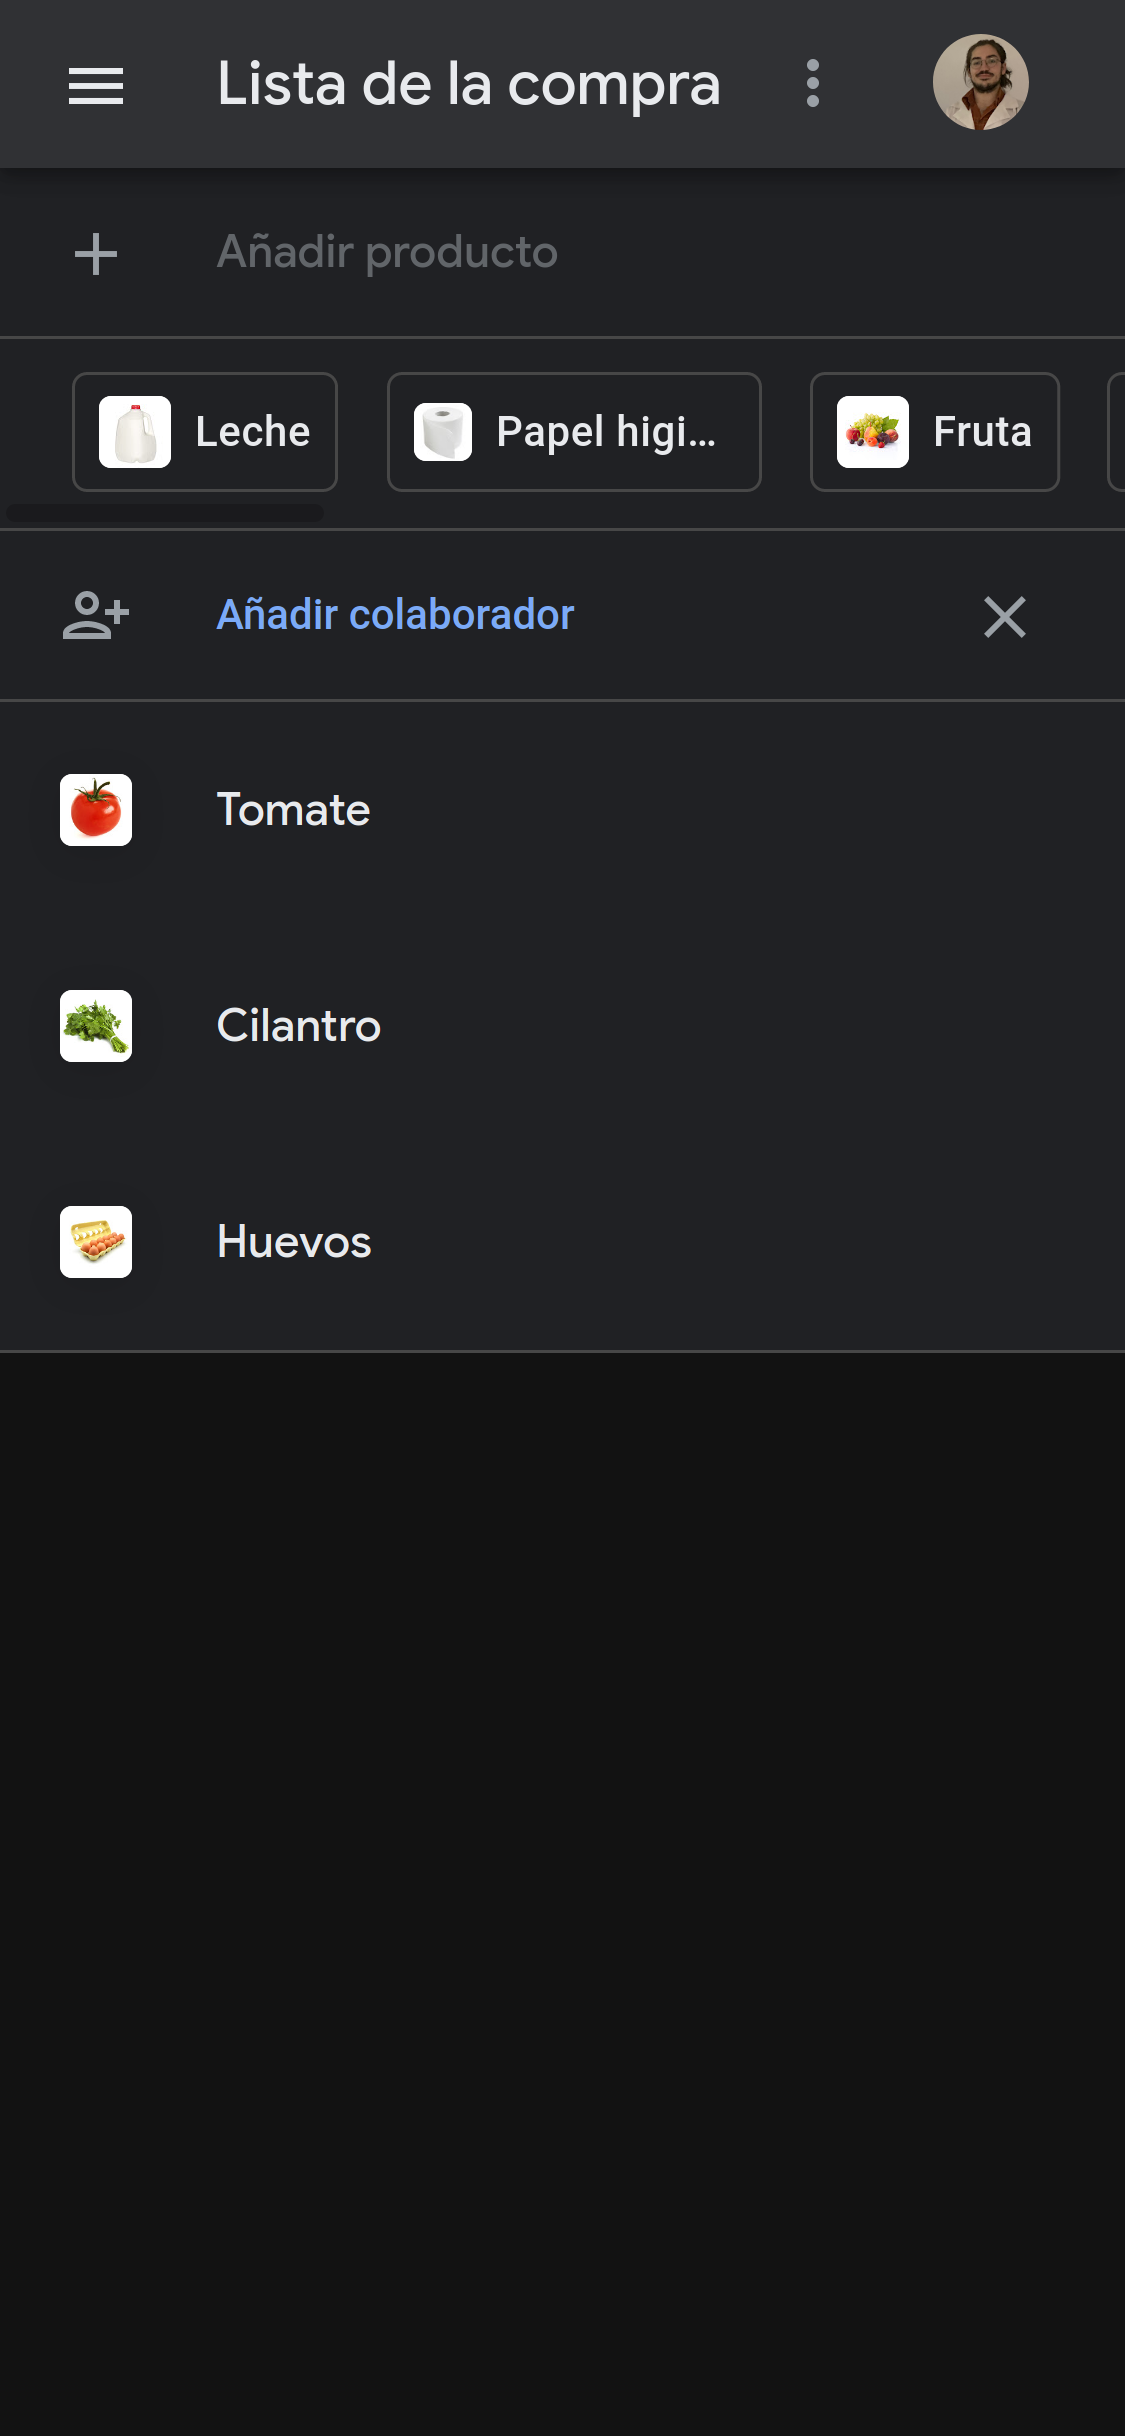
\includegraphics[trim=0 800 0 0, clip, width=.8\textwidth]{images/Screenshot_2020-11-09 Google Shopping List.png}
\end{minipage}
\section{Aplicaciones encontradas que son competencia parcial}
\section{Tablas de aplicaciones y funcionalidades}
\begin{tabular}{@{}rcccccccc@{}}
\textbf{Aplicación} & 
\rotatebox{90}{\textbf{Inventario}} &
\rotatebox{90}{\textbf{Crear listas}} &
\rotatebox{90}{\textbf{Compartir listas}} & 
\rotatebox{90}{\textbf{Notificaciones}} &
\rotatebox{90}{\textbf{Añadir fotos}} & 
\rotatebox{90}{\textbf{Añadir Precios}} &
\rotatebox{90}{\textbf{Categorías}} & 
\rotatebox{90}{\textbf{Voz}} \\
\toprule
Google Shopping List & \xmark & \cmark & \cmark & \xmark & \xmark & \xmark & \xmark & ? \\
\rowcolor{black!15}
Listonic             & \xmark & \cmark & \cmark & \cmark & \cmark & \cmark & \cmark & ? \\
\bottomrule
\end{tabular}

\begin{enumerate}
    \item Google Assistant
    \item Alexa
\end{enumerate}